\documentclass[a4paper]{ctexrep}
\usepackage{listings, graphicx, color, soul, xcolor, bm, geometry, fancyhdr, makeidx,CJK, fontspec, amsmath, savesym}
\usepackage[colorinlistoftodos]{todonotes}
\usepackage[colorlinks,linkcolor=black]{hyperref}
\setmonofont[Mapping={}]{Monaco}	%英文引号之类的正常显示,相当于设置英文字体
\setsansfont{Monaco} %设置英文字体 Monaco, Consolas,  Fantasque Sans Mono
\setmainfont{Monaco} %设置英文字体
% \setCJKmainfont{方正兰亭黑简体}  %中文字体设置
% \setCJKsansfont{华康少女字体} %设置中文字体
% \setCJKmonofont{华康少女字体} %设置中文字体

% \savesymbol{iint}
% \usepackage{txfonts} % txfonts包和amsmath包中的\iint符号冲突,需要先用savesym包保存符号后还原
% \restoresymbol{TXF}{iint}


\definecolor{mygreen}{rgb}{0,0.6,0}
\definecolor{mygray}{rgb}{0.5,0.5,0.5}
\definecolor{mymauve}{rgb}{0.58,0,0.82}
\lstset{ %
backgroundcolor=\color{white},   % choose the background color
basicstyle=\footnotesize\ttfamily,        % size of fonts used for the code
columns=fullflexible,
breaklines=true,                 % automatic line breaking only at whitespace
captionpos=b,                    % sets the caption-position to bottom
tabsize=4,
commentstyle=\color{mygreen},    % comment style
escapeinside={\%*}{*)},          % if you want to add LaTeX within your code
keywordstyle=\color{blue},       % keyword style
stringstyle=\color{mymauve}\ttfamily,     % string literal style
frame=single,
rulesepcolor=\color{red!20!green!20!blue!20},
% identifierstyle=\color{red},
language=c++,
}

\newcommand{\HRule}{\rule{\linewidth}{0.5mm}} % Defines a new command for the horizontal lines,
\geometry{left=3cm,right=3cm,top=3cm,bottom=3cm}
\makeindex
\pagestyle{headings}
\pagestyle{fancy}
\fancyhf{}
\fancyhead[C]{\textbf{By Netcan}}
\fancyhead[R]{\leftmark}
\fancyfoot[ER,OR]{\normalsize\thepage}

\begin{document}

\begin{titlepage}
\newgeometry{top=6.4cm}
\begin{center}
\includegraphics{acm_icpc_logo.png}\\[0.5cm]
\HRule\\[0.4cm]
{\huge \bfseries ACM-ICPC Template Libraries}\\[0.2cm]
\HRule\\[1.5cm]
\textsc{\large 合肥工业大学宣城校区}\\[1cm]
\includegraphics[width=3cm, height=3cm]{hfut_logo.jpg}\\[0.5cm]
Author: \textbf{\emph{Netcan}}\\
Blog: \textbf{\emph{\url{http://www.netcan.xyz}}}\\
{\large \today}\\[2cm]
\end{center}
\end{titlepage}

\tableofcontents

\chapter{数学}
\section{$0-20$的阶乘}
\begin{lstlisting}
const long long fac[21]={1,1,2,6,24,120,720,5040,40320,362880,
						3628800,39916800,479001600,6227020800,
						87178291200,1307674368000,20922789888000,
						355687428096000,6402373705728000,121645100408832000,
						2432902008176640000};
\end{lstlisting}
\section{错排公式}
有n个元素的排列,若一个排列中所有的元素都不在自己原来的位置上,错排数记为$D(n)$,则
$$D(n) = (n-1)[D(n-1)+D(n-2)]$$
\section{最小公倍数$lcm(a,b)$ \&\& 最大公约数$gcd(a,b)$}
\begin{lstlisting}
inline int gcd(int a, int b) { // 如果a<b,则递归得gcd(b,a%b)即gcd(b, a),即交换了位置,时间复杂度O(log max(a, b))
	return b==0?a:gcd(b,a%b)
}
inline int lcm(int a, int b) {
	return a/gcd(a,b)*b;
}
\end{lstlisting}
\section{扩展欧几里得}
求解$a x + b y = gcd(a, b)$
这里得到的是一组$(x, y)$的可行解,$(x+k b, y-k a)$为解集。
\begin{lstlisting}
int extgcd(int a, int b, int &x, int &y) { // x, y为解,返回gcd(a, b)
	int d = a;
	if(b!=0) {
		d = extgcd(b, a%b, y, x);
		y -= (a/b)*x;
	}
	else  {
		x = 1; y = 0;
	}
	return d;
}
\end{lstlisting}



\section{母函数}
$G(x)=(1+x+x^2+\dots+x^N)(1+x^2+x^4+\dots+x^N)\dots(1+x^N)$展开后$x^N$的系数\underline{(注意溢出)}\\
%\begin{lstlisting}
%\end{lstlisting}
\begin{lstlisting}
int c1[MAX_N], c2[MAX_N]; // c1表示每一项的的系数,c2表示每个表达式的临时系数
for(int i=0; i<=N; ++i) { // 每一项应该初始化为1,即1+x+x^2+...+x^N
	c1[i] = 1;
	c2[i] = 0;
}
for(int i=2; i<=N; ++i) { // 从第二个表达式开始
	for(int j=0; j<=N; ++j) // 表示第一个表达式的第j项
		for(int k=0;k+j<=N;k+=i) // k表示后一个表达式的第k项
			c2[j+k] += c1[j]; // 这里应该是相当于C1*x^j * x^k=C1*x^(j+k),即c2[k+j]+=C1[j]
	for(int j=0; j<=N; ++j) {
		c1[j] = c2[j]; // 确定x^j的系数
		c2[j] = 0;
	}
}
\end{lstlisting}
\section{动态规划}
\subsection{最长公共子序列}
$$
dp[i+1][j+1]=\begin{cases}
	dp[i][j]+1 & s1[i]=s2[j] \cr
	max(dp[i+1][j], dp[i][j+1]) & s1[i] \neq s2[j]
\end{cases}
$$
$$
op[i+1][j+1]=\begin{cases}
	\nwarrow & s1[i]=s2[j] \cr
	\uparrow & dp[i][j+1] \geq dp[i+1][j] \cr
	\leftarrow & dp[i][j+1] < dp[i+1][j] \cr
\end{cases}
$$
\subsection{最长上升子序列}
$$dp[i]=max\{1, dp[j]+1 | j<i \&\& a_j<a_i\}$$
$O(N^2)$算法

\begin{lstlisting}
int a[MAX_N], dp[MAX_N]; // a为序列, dp[i]为以a[i]为结尾的最长上升子序列长度
int Maxlis = 0; // 最长上升子序列长度
int n; // a的有效长度
for(int i=0; i<n; ++i) {
	dp[i] = 1; // 记得初始化为1
	for(int j=0; j<i; ++j)
		if(a[i] > a[j])
			dp[i] = max(dp[i], dp[j] + 1);
	Maxlis = max(Maxlis, dp[i]); // 记得更新Maxlis
}
\end{lstlisting}
$O(n log(n))$算法

\begin{lstlisting}
#define INF 0x3f3f3f3f
int a[MAX_N], dp[MAX_N]; // a为序列, dp[i]存放长度为i+1的上升序列中末尾元素的最小值
int n; // 序列长度
memset(dp, 0x3f, sizeof(dp)); // 初始化dp[i]值都为INF
for(int i=0; i<n; ++i)
	*lower_bound(dp, dp+n, a[i]) = a[i];
// cout << lower_bound(dp, dp+n, INF) - dp << endl; // 最长上升序列的长度
\end{lstlisting}

$lower\_bound(dp, dp+n, k)$这个函数从已经排序好的序列$dp$中,二分搜索找出满足$dp_i \ge k$的$dp_i$的最小指针。

$upper\_bound(dp, dp+n, k)$这个函数则从已经排序好的序列$dp$中,二分搜索找出满足$dp_i > k$的$dp_i$的最小指针。

例如求有序数组$a$中的$k$的个数,可以利用下面的代码求出:
\begin{lstlisting}
upper_bound(a, a+n, k) - lower_bound(a, a+n, k)
\end{lstlisting}





\section{高精度}
\subsection{加法\&\&乘法}
适合大数的加法和乘法
\begin{lstlisting}
struct BigInt {
	const static int nlen = 4; // 控制每个数组数字长度,默认为4,计算乘法的时候每个数组相乘也不会溢出int范围
	const static int mod = 10000; // 值为10^nlen
	short n[1000], len;  // 最多存4*1000位长度,可调,short占的内存小,但是速度慢
	BigInt() {
		memset(n, 0, sizeof(n));
		len = 1;
	}
	BigInt(int num) {
		len = 0;
		while(num >0) {
		n[len++] = num%mod;
		num/=mod;
		}
	}
	BigInt(const char *s) {
		int l = strlen(s);
		len = l % nlen  == 0 ? l/nlen : l/nlen+1;
		int index = 0;
		for(int i=l-1; i>=0; i -= nlen) {
		int tmp = 0;
		int j = i-nlen+1;
		if(j<0) j = 0;
		for(int k=j; k<=i; ++k)
			tmp = tmp*10+s[k]-'0';
		n[index++] = tmp;
		}
	}
	BigInt operator+(const BigInt &b) const { // 加法
		BigInt res;
		res.len = max(len, b.len);
		for(int i=0; i<res.len; ++i) {
		res.n[i] += (i<len ? n[i]:0) + (i<b.len ? b.n[i]:0);
		res.n[i+1] += res.n[i]/mod;
		res.n[i] = res.n[i]%mod;
		}
		if(res.n[res.len] > 0) ++res.len;
		return res;
	}
	BigInt operator*(const BigInt &b) const { // 乘法
		BigInt res;
		for(int i=0; i<len; ++i) { // 类似母函数,第一个数组
		int up = 0; // 进位
		for(int j=0; j<b.len; ++j) { // 第二个数组
			int tmp = n[i]*b.n[j] + up + res.n[i+j]; // 控制nlen=4是防止tmp溢出
			res.n[i+j] = tmp%mod;
			up = tmp/mod;
		}
		if(up!=0)
			res.n[i+b.len] = up;
		}
		res.len = len+b.len;
		while(res.n[res.len-1] == 0 && res.len>1 ) --res.len;
		return res;
	}
	void show() const {
		printf("%d", n[len-1]); // 先输出最高位,后面可能需要前导0
		for(int i=len-2; i>=0; --i)
		printf("%04d", n[i]); // 前导0,%04d和nlen一致
		printf("\n");
	}
};
\end{lstlisting}
\section{素数}
\subsection{埃式筛法 $O(n log logn)$}
\begin{lstlisting}
bool is_prime[MAX_N]; // 第i个素数
int prime[MAX_N+1]; // is_prime[i]为true表示i是素数

int sieve(int n) { // 返回n以内的素数个数
	int p=0;
	memset(is_prime, true, sizeof(is_prime));
	is_prime[0] = is_prime[1] = false;
	for(int i=2; i<=n; ++i) {
		if(is_prime[i]) {
			prime[p++] = i;
			for(int j=2*i; j<=n; j+=i) is_prime[j] = false;
		}
	}
	return p;
}
\end{lstlisting}

\subsection{区间筛法}
筛选出区间$[a, b]$间的素数, $a \ge 1$

\begin{lstlisting}
typedef long long ll;
bool is_prime[MAX_L]; // 对区间[a, b]内的整数筛选,is_prime[i-a] == true表示i是素数, MAX_L = B-A+1
bool is_prime_small[MAX_SQRT_B]; 

void segment_sieve(ll a, ll b) {
	memset(is_prime, true, sizeof(is_prime)); 
	memset(is_prime_small, true, sizeof(is_prime_small));
	if(a == 1) is_prime[0] = false; // 1不是素数

	for(int i=2; (ll)i*i <= b; ++i) {
		if(is_prime_small[i]) {
			for(int j=2*i; (ll)j*j <= b; j+=i) is_prime_small[j] = false; // 筛[2, √b]
			for(ll j = max(2LL, (a+i-1)/i)*i; j<=b; j+=i) is_prime[j-a] = false;
		}
	}
}
\end{lstlisting}

\section{快速幂运算 $O(log n)$}
\begin{lstlisting}
typedef long long ll;
ll mod_pow(ll x, ll n, ll mod) {
	ll res = 1;
	while(n > 0) {
		if(n&1) res = res * x % mod; // 如果最低位为1,则乘上x^(2^i)
		x=x * x % mod; // x平方
		n >>= 1;
	}
	return res;
}
\end{lstlisting}

递归写法:
\begin{lstlisting}
typedef long long ll;
ll mod_pow(ll x, ll n, ll mod) {
	if(n == 0) return 1;
	ll res = mod_pow(x * x % mod, n/2, mod);
	if(n & 1) res = res * x % mod;
	return res;
}
\end{lstlisting}

\chapter{计算几何}
\section{点}


\chapter{组合博弈}
\section{SG函数 \&\& NIM游戏}
\begin{enumerate}
	\item 可选步数为$[1, m]$的连续整数,直接取模即可,$SG(x)=x\%(m+1)$;
	\item 可选步数为任意步,$SG(x)=x$;
\end{enumerate}

步数集合S需排序(升序), sg数组记得初始化,对于确定的步数,一系列sg(x)值也就确定了。

最终判断各个sg(x)的异或和,即可判断胜负。异或和为0先手必败,反之必胜。

\subsection{打表}
\begin{lstlisting}
int S[STEP_N], steps, sg[MAX_N];  // S集合存放走法,steps存放走法数,sg存放sg(x)的值
bool vis[MAX_N]; // 标记
void get_sg(int n) {
	memset(sg, 0, sizeof(sg)); // 初始化sg
	for(int i=1; i<=n; ++i) { // 从sg[1]开始计算
		memset(vis, 0, sizeof(vis)); // 每次计算完一个sg值需要归零
		for(int j=0; S[j] <= i && j <steps ; ++j)
			vis[sg[i-S[j]]] = true; // 标记各个后继节点的sg值
		for(int j=0; j<=n; ++j)
			if(!vis[j]) { // 找出sg补集的最小值
				sg[i] = j;
				break;
			}
	}
}
\end{lstlisting}
\subsection{递归}
\begin{lstlisting}
#pragma comment(linker, "/STACK:1024000000,1024000000") // 防止爆栈
int S[STEP_N], sg[MAX_N], k; // 题目中的步数集合S, 以及sg(t)函数值sg(t), 步数集合大小k

int SG(int p) { // 求sg(t)值函数SG(t)
	bool vis[101] = {false}; // 标记各个sg(t)的值,为了方便求补集最小值(sg(t)),数组不宜开过大,爆栈就扩栈
	for(int i=0; i<k; ++i) {
		int t = p - S[i];
		if(t < 0) // 小于0则退出循环,求出该层的sg(t)值
			break;
		if(sg[t] == -1) // 记得memset(sg, -1, sizeof(sg));
			sg[t] = SG(t); // 递归求sg(t)
		vis[sg[t]] = true; // 标记该层的sg(t)值
	}
	for(int i=0;; ++i) // 求出该层的sg(t)值,即补集的最小值
		if(!vis[i])
			return i;
}
\end{lstlisting}



\chapter{数据结构}
\section{二叉搜索树}
二叉搜索树是能够高效地进行如下操作的数据结构:
\begin{itemize}
		\item 插入一个数值
		\item 查询是否包含某个数值
		\item 删除某个数值
\end{itemize}

时间复杂度:\(O(log(n))\)
\begin{lstlisting}
struct node { // 树节点
		int val;
		node *lch, *rch;
};

node *insert(node *p, int x) { //插入数值x
	if(p == NULL) { // 新建节点插入
		node *q = new node;
		q->val = x;
		q->lch = q->rch = NULL;
		return q;
	}
	else {
		if(x < p->val)	p->lch = insert(p->lch, x); // 往左边搜索
		else	p->rch = insert(p->rch, x); // 往右边搜索
		return p;
	}
}

bool find(node *p, int x) { // 查找数值x
	if(p == NULL) return false; // 找不到
	else if(p->val == x) return true; // 找到
	else if(x < p->val) return find(p->lch, x); // 往左边搜索
	else return find(p->rch, x); // 往右边搜索
}

node *remove(node *p, int x) { // 删除数值x
	if(p == NULL) return NULL; // 找不到数值
	else if(x < p->val) p->lch=remove(p->lch, x); // 往左边搜索
	else if(x > p->val) p->rch=remove(p->rch, x); // 往右边搜索
	else { // 找到
		if(p->lch == NULL) { // 如果删除的节点没有左儿子,将右儿子提上来
			node *q = p->rch;
			delete p; // 删除
			return q;
		}
		else if(p->lch->rch == NULL) { // 如果删除的节点左儿子没有右儿子,将左儿子提上来
			node *q = p->lch;
			q->rch = p->rch;
			delete p; // 删除
			return q;
		}
		else { // 否则,将左儿子的子孙中最大的节点提上来
			node *q;
			for(q=p->lch; q->rch->rch; q=q->rch); // 往左儿子搜索最大节点
			node *r = q->rch; // r指向左儿子最大子孙节点,q指向最大儿子的父亲
			q->rch = r->lch; // 因为r为提上去的节点,将r的左儿子(有的话,否则为NULL)挂到q的右边
			r->lch = p->lch;
			r->rch = p->rch;
			delete p; // 删除
			return r;
		}
	}
	return p;
}
/**************Usage**************/
	node *testbst=NULL; // 初始化
	testbst = insert(testbst, x); // 插入数值x
	if(find(testbst, x)) // 查找数值x
		// balabala
	else
		// balabala
	testbst = remove(testbst, x); // 删除数值x
\end{lstlisting}

\section{并查集}
并查集是一种用来管理元素分组情况的数据结构,可以高效地进行如下两种操作:
\begin{itemize}
		\item 合并两个集合
		\item 查找某元素属于哪个集合
\end{itemize}

时间复杂度:\(O(\alpha(n))\)
\begin{lstlisting}
int par[MAX_N];
// int height[MAX_N];
void init(int n) { // 初始化
	for (int i = 1; i <= n; ++i) {
		par[i] = i;
		// height[i] = 0;
	}
}
int find(int x) { // 查找根节点(集合)+路径压缩
	return x==par[x]?x:par[x]=find(par[x]);
}
void unite(int x, int y) { // 合并集合
	x = find(x);
	y = find(y);
	if(x!=y) {
	par[x] = y;
	// if(height[x] < height[y])
	// par[x] = y;
	// else
	// par[y] = x;
	// if(height[x] == height[y]) ++height[x];
	}
}
bool same(int x,int y) { // 判断两个元素是否同集合
	return find(x) == find(y);
}
\end{lstlisting}


\chapter{字符串}
\section{KMP算法 $O(M+N)$}
\url{http://www.cnblogs.com/goagent/archive/2013/05/16/3068442.html}\\
求出模式串$P$在字符串$S$中的位置
当失配前($P_j \neq S_i$),满足
$$
P_0P_1 \cdots P_{k-1} = S_{i-k}S_{i-k+1} \cdots S_{i-1} 
$$
已有部分匹配结果,
$$
P_{j-k}P_{j-k+1} \cdots P_{j-1} =  S_{i-k}S_{i-k+1} \cdots S_{i-1}
$$
由上两式子可得:
$$
P_0P_1 \cdots P_{k-1} = P_{j-k}P_{j-k+1} \cdots P_{j-1}
$$
定义$next[j] = k$,有
$$
next[j]=\begin{cases}
	-1 & j=0\cr
	max\{k|0<k<j \ \&\&\  P_0P_1 \cdots P_{k-1} = P_{j-k}P_{j-k+1} \cdots P_{j-1}\}\cr
	0 & Other \  Conditions\cr
\end{cases}
$$
\begin{lstlisting}
int Next[MAX_PLEN];
string s, p; // 求出模式串p在字符串s中的位置
void getNext() {
	Next[0] = -1;
	int i=0, j=-1;
	while(i!=p.length()-1) {
		if(j == -1 || p[j] == p[i]) {
			++i;
			++j;
			Next[i] = p[i] != p[j]?j:Next[j];
		}
		else
			j = Next[j];
	}
}

int kmp(const int sIndex = 0) // 返回模式串位置
{
	getNext();
    int i = sIndex, j = 0;
    while(i != s.length() && j != p.length()) {
        if (j == -1 || s[i] == p[j]) {
            ++i;
            ++j;
        }
        else
            j = next[j];
    }
    return j == p.length() ? i - j: -1;
}
\end{lstlisting}


\section{字典树}
\url{http://www.cnblogs.com/tanky_woo/archive/2010/09/24/1833717.html} \\
\begin{lstlisting}
const int MAX_C = 26; // 假设全为小写字母
struct Trie {
	Trie *next[MAX_C];
	int v; // 存放以此为前缀的个数
	void init() {
		for(int i=0; i<MAX_C; ++i) next[i] = NULL;
	}
};
Trie *root = new Trie;
root->init(); // 记得初始化,因为堆上的内存是随机的

void createTrie(const string &str) { // 建立字典树
	Trie *p = root, *q;
	for(int i=0; i<str.length(); ++i) {
		int id = str[i] - 'a';
		if(p->next[id] == NULL) {
			q = new Trie;
			q->v = 1;
			q->init();
			p->next[id] = q;
			p = p->next[id];
		}
		else {
			++(p->next[id]->v);
			p = p->next[id];
		}
	}
	// p->v = -1; // 结尾
}

int findTrie(const string &w) { // 查找字典树
	Trie *p = root;
	for(int i=0; i<w.length(); ++i) {
		int id = w[i] - 'a';
		p = p->next[id];
		if(p == NULL) return 0; // 空集,则不存在以此为前缀的串
	}
	return p->v; // 此字符串是字符集某串的前缀
}

void freeTrie(Trie *p) { // 释放内存
	if(p == NULL) return;
	for(int i=0; i<MAX_C; ++i) freeTrie(p->next[i]);
	delete p;
}


\end{lstlisting}

\chapter{图}
\section{邻接表}
\subsection{样例1}
\begin{lstlisting}
#define MAX_V 100
vector<int> G[MAX_V];

/* 边上有属性
 * struct edge { int to, cost; };
 * vector<edge> G[MAX_V];
 */

int main()
{
	int V, E;
	cin >> V >> E;
	for(int i=0; i<E; ++i) {
		int s, t;
		cin >> s >> t;
		G[s].push_back(t); // s->t
		// G[s].push_back(edge(t, c));
		// G[t].push_back(s); // 无向图
	}
	// balabala...
}
\end{lstlisting}


\subsection{样例2}
\section{单源最短路}
\subsection{Bellman-Ford算法$O(V*E)$}
\begin{lstlisting}
struct Edge{ // 边
	int from, to, cost; // 顶点from指向to权值为cost
} edge[MAX_E];
int d[MAX_V];
int V, E;  // 节点数量V, 边的数量E

bool bellman_ford(int s) { // 求解顶点s出发到所有节点的最短距离
	memset(d, 0x3f, sizeof(d)); // 初始化到INF
	d[s] = 0;
	for(int i=1; i<=V-1; ++i) // 图的顶点编号从1开始计算
		for(int j=1; j<=E; ++j) {
			Edge e=edge[j];
			if(d[e.to] > d[e.from] + e.cost) // 松弛计算
				d[e.to] = d[e.from] + e.cost;
		}

	int flag = true; // 判断有没有负圈
	for(int j=1; j<=E; ++j)
		if(d[edge[j].to] > d[edge[j].from] + edge[j].cost) {
			flag = false;
			break;
		}
	return flag;
}
\end{lstlisting}

\subsection{Dijkstra算法}
$O(V^2)$
\begin{lstlisting}
int cost[MAXV][MAXV]; // cost[u][v]表示e={u,v}的权值(不存在则INF)
int d[MAXV]; // 顶点s出发的最短距离
bool used[MAXV]; // 标记已经使用过的顶点
int V, E; // 顶点数V,边数E

void dijkstra(int s) { // 源点s
	memset(d, 0x3f, sizeof(d)); // 初始化至INF
	memset(used, 0, sizeof(used)); // 初始化至INF
	d[s] = 0;

	while(true) {
		int v = -1;
		for(int u=1; u<=V; ++u) // 从未使用过的节点中选择一个距离最小的顶点,编号从1开始
			if(!used[u] && (v==-1 || d[u] < d[v])) v = u;
		if(v == -1) break; // 已经用完所有顶点了
		used[v] = true; // 标记顶点
		for(int u=1; u<=V; ++u) // 顶点编号从1开始计算
			d[u] = min(d[u], d[v]+cost[v][u]);
	}
}
\end{lstlisting}

% \clearpage
$O(E logV)$
\begin{lstlisting}
struct edge { // 顶点属性
	int to, val;
	edge(int t, int v): to(t), val(v){}
	bool operator<(const edge &b) const {
		return val > b.val;
	}

};
vector<edge> G[MAX_V]; // 邻接链表图
int d[MAX_V];
int V, E; // 顶点数V, 边数E

void dijkstra(int s) {
	priority_queue<edge> que;
	memset(d, 0x3f, sizeof(d));
	d[s] = 0;
	que.push(edge(s, 0)); // 源点入队

	while(!que.empty()) {
		edge p = que.top(); que.pop();
		int v = p.to;
		if(d[v] < p.val) continue; // 当前最小值不是最短距离的话,丢弃
		for(int i=0; i<G[v].size(); ++i) {
			edge e = G[v][i];
			if(d[e.to] > d[v] + e.val) {
				d[e.to] = d[v] + e.val;
				que.push(edge(e.to, d[e.to]));
			}
		}
	}
}
\end{lstlisting}



\subsection{差分约束系统}
如果一个系统由n个变量和m个约束条件组成,其中每个约束条件形如$x_j-x_i \le b_k$ $(i,j \in [1,n],k \in [1,m])$,则称其为差分约束系统(system of difference constraints)。亦即,差分约束系统是求解关于一组变量的特殊不等式组的方法。

求解差分约束系统,可以转化成图论的单源最短路径(或最长路径)问题。

观察$x_j-x_i \le b_k$,会发现它类似最短路中的三角不等式 $d[v] \le d[u]+w[u,v]$,即$d[v]-d[u] \le w[u,v]$。因此,以每个变量$x_i$为结点,对于约束条件$x_j-x_i<=b_k$,连接一条边$(i,j)$,边权为$b_k$。我们再增加一个源点s,s与所有定点相连,边权均为0。对这个图,以s为源点运行Bellman-ford算法(或SPFA算法),最终${d[i]}$即为一组可行解。

例如:
$$
\begin{cases}
   b-a \le 3  & (1)\cr
   c-b \le 2  & (2)\cr
   c-a \le 4 & (3)\cr
\end{cases}
$$

求出c-a的最大值。

建立如下有向图
\begin{center}
	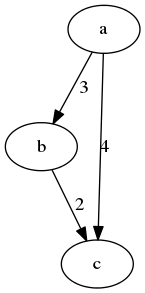
\includegraphics[width=3cm] {sodc.png}
\end{center}

根据条件有

$$
\begin{cases}
c-a \le 4 & (4)\cr
c-a \le 3+2 = 5 & (5) \cr
\end{cases}
$$

最短路即为c-a的最大值,即4。






\section{任意两点间的最短路}
Floyd $O(V^3)$
$$
d[i][j] = min(d[i][j], d[i][k] + d[k][j])
$$

和Bellman-Ford算法一样可以处理负圈,只需检查d[i][i]是否负数的顶点即可。

\begin{lstlisting}
int V, E; // 顶点数V, 边数E
int d[102][102]; // d[u][v]表示边e={u, v}的权值(不存在则设为INF, d[u][u]=0)

void floyd() {
	for(int k=0; k<V; ++k) // 顶点依次从0-V-1开始
		for(int i=0; i<V; ++i)
			for(int j=0; j<V; ++j)
				d[i][j] = min(d[i][j], d[i][k]+d[k][j]); // i到j的最短距离等于i到j的距离与i到k和k到j的距离的最小值
	return;
}
\end{lstlisting}
\section{最小生成树}
\subsection{Prim算法 $O(V^2)$}
\begin{lstlisting}
int cost[MAX_V][MAX_V]; // cost[u][v]表示边e=(u, v)的权值(不存在则INF)
int mincost[MAX_V]; // 从集合出发的边到每个顶点的最小权值
bool used[MAX_V]; // 顶点u是否在集合中
int V; // 顶点数

int prim() {
	int res = 0;
	memset(used, 0, sizeof(used));
	memset(mincost, 0x3f, sizeof(mincost));
	mincost[0] = 0;
	while(true) {
		int v = -1;
		for(int u=0; u<V; ++u)
			if(!used[u] && ( v==-1 || mincost[u] < mincost[v])) v = u;
		if(v == -1) break;
		used[v] = true; // 标记顶点到集合中
		res += mincost[v];
		for(int u=0; u<V; ++u)
			mincost[u] = min(mincost[u], cost[v][u]);
	}
	return res;
}
\end{lstlisting}

\subsection{Kruskal算法 $O(E log(V))$}
\begin{lstlisting}
int V, E; // 边数,顶点数
struct edge { // 边
	int u, v, cost;
	bool operator<(const edge &b) const {
		return cost < b.cost; // 需要按照边的权值从小到大的顺序排序
	}
} es[MAX_E];

int kruskal() {
	sort(es, es+E); // 排序
	init_union_find(V); // 初始化并查集
	int res = 0;
	for(int i=0; i<E; ++i) {
		edge e = es[i];
		if(find(e.u) != find(e.v)) { // 判断是否产生圈(重边也算在内)
			unite(e.u, e.v);
			res+=e.cost;
		}
	}
	return res;
}
\end{lstlisting}

\end{document}
